\documentclass[UTF8,a4paper,10pt,nocolorlinks]{ctexbook}

\usepackage[left=2.50cm, right=2.50cm, top=2.50cm, bottom=2.50cm]{geometry} %页边距
\CTEXsetup[format={\Large\bfseries}]{section} %设置章标题居左   
\usepackage{ctex}
\CTEXoptions[today=old]
\usepackage{cite}
\usepackage{textcomp}
\usepackage{listings}
\usepackage{xcolor}
\usepackage{varioref}
\usepackage{ctex}
\usepackage{multicol}
\usepackage{amssymb} 
\usepackage{setspace}
\usepackage{tikz} 
\usepackage{mdframed}
\usepackage{titletoc}
\usepackage{etoolbox}

\usepackage{helvet}
\usepackage{caption}
\usepackage{multicol} 
\usepackage{changepage}
\usepackage{graphics}
\usepackage{amsmath, amsfonts, amssymb}
\usepackage[english]{babel}
\usepackage{color}      
\usepackage{graphicx}   
\usepackage{url}        
\usepackage{bm}         
\usepackage{multirow}
\usepackage{booktabs}
\usepackage{epstopdf}
\usepackage{epsfig}
\usepackage{algorithm}
\usepackage{algorithmic}
\usepackage{listings}  % 代码框


\usepackage{listings}
\usepackage{color}

\definecolor{dkgreen}{rgb}{0,0.6,0}
\definecolor{gray}{rgb}{0.5,0.5,0.5}
\definecolor{mauve}{rgb}{0.58,0,0.82}

\lstset{ %
  language=C++,                % the language of the code
  basicstyle=\footnotesize,           % the size of the fonts that are used for the code
  numbers=left,                   % where to put the line-numbers
  numberstyle=\tiny\color{gray},  % the style that is used for the line-numbers
  stepnumber=1,                   % the step between two line-numbers. If it's 1, each line 
                                  % will be numbered
  numbersep=5pt,                  % how far the line-numbers are from the code
  backgroundcolor=\color{white},      % choose the background color. You must add \usepackage{color}
  showspaces=false,               % show spaces adding particular underscores
  showstringspaces=false,         % underline spaces within strings
  showtabs=false,                 % show tabs within strings adding particular underscores
  frame=single,                   % adds a frame around the code
  rulecolor=\color{black},        % if not set, the frame-color may be changed on line-breaks within not-black text (e.g. commens (green here))
  tabsize=2,                      % sets default tabsize to 2 spaces
  captionpos=b,                   % sets the caption-position to bottom
  breaklines=true,                % sets automatic line breaking
  breakatwhitespace=false,        % sets if automatic breaks should only happen at whitespace
  title=\lstname,                   % show the filename of files included with \lstinputlisting;
                                  % also try caption instead of title
  keywordstyle=\color{blue},          % keyword style
  commentstyle=\color{dkgreen},       % comment style
  stringstyle=\color{mauve},         % string literal style
  escapeinside={\%*}{*)},            % if you want to add LaTeX within your code
  morekeywords={*,...}               % if you want to add more keywords to the set
}


\usepackage[pagestyles]{titlesec}
\renewcommand{\algorithmicensure}{ \textbf{Input:}} 
\renewcommand{\figurename}{图}
\newcommand{\upcite}[1]{\textsuperscript{\textsuperscript{\cite{#1}}}}

\newpagestyle{teststyle}{
  \sethead{\emph{姓名:冯学伟}}{\emph{\sectiontitle}}{\emph{第\thepage页}}
  \renewcommand{\makeheadrule}{
    \makebox[0pt][l]{\rule[-.3\baselineskip]{\linewidth}{.5pt}}
    \rule[-.4\baselineskip]{\linewidth}{.5pt}
  }
}
\usepackage{color}
\usepackage{subfigure}
\usepackage{changepage}
\usepackage{fancyhdr}   %设置页眉、页脚
\pagestyle{fancy}       %%%单线页眉
\fancyhead{}
\fancyhead[LO]{\emph{姓名:冯学伟}}
\fancyhead[RO]{\emph{第\thepage页}}
\fancypagestyle{plain}{
  \pagestyle{fancy}
}
\usepackage{shorttoc}
\usepackage{xcolor}
\usepackage{mdframed}
\usepackage{titletoc}

\DeclareRobustCommand{\chuhao}{\fontsize{42pt}{\baselineskip}\selectfont}  % 初号
\DeclareRobustCommand{\xiaochu}{\fontsize{36pt}{\baselineskip}\selectfont} % 小初
\DeclareRobustCommand{\yihao}{\fontsize{26pt}{\baselineskip}\selectfont}   % 一号
\DeclareRobustCommand{\xiaoyi}{\fontsize{24pt}{\baselineskip}\selectfont}  % 小一
\DeclareRobustCommand{\erhao}{\fontsize{22pt}{\baselineskip}\selectfont}   % 二号
\DeclareRobustCommand{\xiaoer}{\fontsize{18pt}{\baselineskip}\selectfont}  % 小二
\DeclareRobustCommand{\sanhao}{\fontsize{16pt}{\baselineskip}\selectfont}  % 三号 
\DeclareRobustCommand{\xiaosan}{\fontsize{15pt}{\baselineskip}\selectfont} % 小三
\DeclareRobustCommand{\sihao}{\fontsize{14pt}{\baselineskip}\selectfont}   % 四号
\DeclareRobustCommand{\xiaosi}{\fontsize{12pt}{\baselineskip}\selectfont}  % 小四
\DeclareRobustCommand{\wuhao}{\fontsize{10.5pt}{\baselineskip}\selectfont} % 五号
\DeclareRobustCommand{\xiaowu}{\fontsize{9pt}{\baselineskip}\selectfont}   % 小五
\DeclareRobustCommand{\liuhao}{\fontsize{7.5pt}{\baselineskip}\selectfont} % 六号
\DeclareRobustCommand{\xiaoliu}{\fontsize{6.5pt}{\baselineskip}\selectfont}% 小六
\DeclareRobustCommand{\qihao}{\fontsize{5.5pt}{\baselineskip}\selectfont}  % 七号

\lstset{numbers=left,numberstyle=\tiny,
breaklines=true,  %代码过长则换行
keywordstyle=\color{blue!70},commentstyle=\color{red!50!green!50!blue!50},frame=shadowbox, rulesepcolor=\color{gray!20!green!20!blue!20},escapeinside=``,xleftmargin=2em,xrightmargin=2em, aboveskip=1em}

\providecommand{\keywords}[1]{\textbf{\textit{keywords---}} #1}

% 设置章节格式
% 一级标题:黑体,三号,加粗;间距:段前 0.5 行,段后 1 行;
% \ctexset{chapter={
%     name = {第,章},
%     number = {\arabic{chapter}},
%     format = {\heiti \bfseries \centering \zihao{3}},
%     aftername = \hspace{9bp},
%     pagestyle = BIThesis,
%     beforeskip = 8bp,
%     afterskip = 32bp,
%     fixskip = true,
%   }
% }

% % 二级标题:黑体,四号,加粗;间距:段前 0.5 行,段后 0 行;
\ctexset{section={
    number = {\thechapter.\hspace{4bp}\arabic{section}},
    format = {\heiti \raggedright \bfseries \zihao{4}},
    aftername = \hspace{8bp},
    beforeskip = 20bp plus 1ex minus .2ex,
    afterskip = 18bp plus .2ex,
    fixskip = true,
  }
}

% % 三级标题:黑体、小四、加粗;间距:段前 0.5 行,段后 0 行;
\ctexset{subsection={
    number = {\thechapter.\hspace{3bp}\arabic{section}.\hspace{3bp}\arabic{subsection}},
    format = {\heiti \bfseries \raggedright \zihao{-4}},
    aftername = \hspace{7bp},
    beforeskip = 17bp plus 1ex minus .2ex,
    afterskip = 14bp plus .2ex,
    fixskip = true,
  }
}

% 设置目录样式
% 添加 PDF 链接
\addtocontents{toc}{\protect\hypersetup{hidelinks}}

% 解决「目录」二字的格式问题
\renewcommand{\contentsname}{
  \fontsize{16pt}{\baselineskip}
  \normalfont\heiti{目~~~~录}
  \vspace{-8pt}
}
% 定义目录样式
\titlecontents{chapter}[0pt]{\songti \zihao{-4}}
{\thecontentslabel\hspace{\ccwd}}{}
{\hspace{.5em}\titlerule*{.}\contentspage}
\titlecontents{section}[2\ccwd]{\songti \zihao{-4}}
{\thecontentslabel\hspace{\ccwd}}{}
{\hspace{.5em}\titlerule*{.}\contentspage}
\titlecontents{subsection}[4\ccwd]{\songti \zihao{-4}}
{\thecontentslabel\hspace{\ccwd}}{}
{\hspace{.5em}\titlerule*{.}\contentspage}

\usepackage{hyperref} %bookmarks
% \usepackage[colorlinks,linkcolor=red,anchorcolor=blue,citecolor=green,CJKbookmarks=True]{hyperref}
\hypersetup{colorlinks, bookmarks, unicode} % unicode
 
\captionsetup[figure]{labelfont={bf},labelformat={default},labelsep=period,name={图}}
\newenvironment{figurehere}
{\def\@captype{figure}}
{}

\title{
    \huge{\textbf{Working Summary}}
}

\author{fengxuewei}
\date{\today}

\begin{document}
    % \maketitle
    \tableofcontents
    \pagestyle{teststyle}  
  % 软件总体要求
  \chapter{引言}
    \section{项目背景}
    \section{总体要求}
  \clearpage
  % 软件开发
    % (几个主要的类型 + 软件仿真)
  \chapter{软件开发}
    \section{需求分析}
        \subsection{功能需求}
        \subsection{系统功能图}
        这个阶段的任务仍然不是具体地解决问题,而是准确地确定“为了解决这个问题,目标系统必须做什么”,主要是确定目标系统必须具备哪些功能。
    \par 用户了解他们所面对的问题,知道必须做什么,但是通常不能完整准确地表达出他们的要求,更不知道怎样利用计算机解决他们的问题;软件开发人员知道怎样使 用软件实现人们的要求,但是对特定用户的具体要求并不完全清楚。因此系统分析员在需求分析阶段必须和用户密切配合,充分交流信息,以得出经过用户确认的系 统逻辑模型。通常用数据流图、数据字典和简要的算法描述表示系统的逻辑模型。
    在需求分析阶段确定的系统逻辑模型是以后设计和实现目标 系统的基础,因此必须准确完整地体现用户的要求。系统分析员通常都是计算机软件专家,技术专家一般都喜欢很快着手进行具体设计,然而,一旦分析员开始谈论 程序设计的细节,就会脱离用户,使他们不能继续提出他们的要求和建议。较件工程使用的结构分析设计的方法为每个阶段都规定了特定的结束标准,需求分析阶段 必须提供完整准确的系统逻辑模型,经过用户确认之后才能进入下一个阶段,这就可以有效地防止和克服急于着手进行具体设计的倾向。
    
    \section{概要设计}
        \subsection{基本数据流程}
        \subsection{系统功能模块划分、功能分配}
        \subsection{数据结构设计}
            \subsubsection{实体对象关系设计}
            \subsubsection{E-R图到关系模式}
        
    这个阶段必须回答的关键问题是:“概括地说,应该如何解决这个问题?”
    首先,应该考虑几种可能的解决方案。列如,目标系统的一些主要功能是用计算机自动完成还是用人工完成;如果使用计算机,那么是使用批处理方式还是人机交互方式;信息存储使用传统的文件系统还是数据库……。通常至少应该考虑下述几类可能的方案:
    低成本的解决方案。系统只能完成最必要的工作,不能多做一点额处的工作。
    中等成本的解决方案。这样的系统不仅能够很好地完成预定的任务,使用起来很方便,而且可能还具有用户没有具体指定的某些功能和特点。虽然用户没有提出这些具体要求,但是系统分析员根据自己的知识和经验断定,这些附加的能力在实践中将证明是很有价值的。
    高成本的“十全十美”的系统。这样的系统具有用户可能希望有的所有功能和特点。
    系统分析员应该使用系统流程图或其他工具描述每种可能的系统,估计每种方案的成本和效益,还应该在充分权衡各种方案的利弊的基础上,推荐一个较好的系统 (最佳方案),并且制定实现所推荐的系统的详细计划。如果用户接受分析员推荐的系统,则可以着手完成本阶段的另一项主要工作。
    上面的 工作确定了解决问题的策略以及目标系统需要哪些程序,但是,怎样设计这些程序呢?结构设计的一条基本原理就是程序应该模块化,也就是一个大程序应该由许多 规模适中的模块按合理的层次结构组织而成。总体设计阶段的第二项主要任务就是设计软件的结构,也就是确定程序由哪些模块组成以及模块间的关系。通常用层次 图或结构图描绘软件的结构。


    \section{详细设计}
    \subsection{导航控制器}
    \subsection{制导控制器}
    \subsection{姿态控制器}
    \subsection{数据流}
    总体设计阶段以比较抽象概括的方式提出了解决问题的办法。详细设计阶段的任务就是把解法具体化,也就是回答下面这个关键问题:“应该怎样具体地实现这个系统呢?”
  这个阶段的任务还不是编写程序,而是设计出程序的详细规格说明。这种规格说明的作用很类似于其他工程领域中工程师经常使用的工程蓝图,它们应该包含必要的细节,程序员可以根据它们写出实际的程序代码。
  通常用HIPO图(层次图加输入/处理/输出图)或PDL语言(过程设计语言)描述详细设计的结果。

    \section{编码和单元测试}
  这个阶段的关键任务是写出正确的容易理解、容易维护的程序模块。\par
  程序员应该根据目标系统的性质和实际环境,选取一种适当的高级程序设计语言(必要时用汇编语言),把说细设计的结果翻译成用选定的语言书写的程序,并且仔细测试编写出的每一个模块。

  \clearpage
  \chapter{算法}
    \section{导航控制-路径管理}
            \subsection{航点控制逻辑1}
在引入算法之前,我们需要先了解一个概念"半平面(half-plane)",
半平面是被用来指定是否航点切换的核心条件,
通过无人机当前位置和半平面的几何关系,来判定航点是到达。具体的几何关系式如下:
    \begin{equation} % 等式
        \begin{aligned}
            \textit{H}(r,n) = \left\{ p \in R^{3} : \left(p-r\right)^{T}n \geq 0 \right\} 
        \end{aligned}
    \end{equation}
    \par 其中的 $r$ 为正在执行的目标航点,$n$为该半平面的法向量,$p$为无人机的当前位置,物理模型如图\ref{half_plane}所示。定义了一个单位向量$q_{i}$和 $n_{i}$,
    $q_{i}$ 是航线 $\overline{w_{i}w_{i+1}}$ 的单位方向向量,所以存在一个三维向量$n_{i}$,可以把航线 $\overline{w_{i-1}w_{i}}$ 和 $\overline{w_{i}w_{i+1}}$ 分隔开.
    \begin{equation}
        \begin{cases}
        &q_{i} \triangleq \frac{w_{i+1}-w_{i}}{\lVert w_{i+1}-w_{i} \rVert} \\
        &n_{i} \triangleq \frac{q_{i-1}+q_{i}}{\lVert q_{i-1}+q_{i} \rVert}
        \end{cases}
    \end{equation}
    \begin{figure}[b]
        \centering
        \subfigure[]{
            \begin{minipage}[t]{0.48\linewidth}
                \centering
                    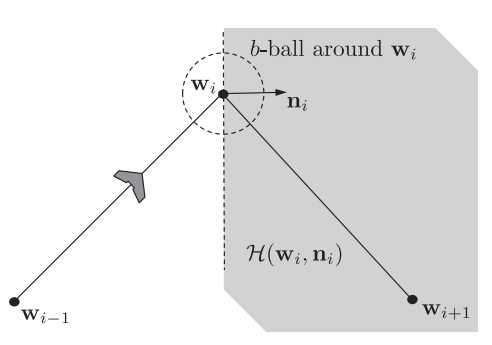
\includegraphics[width=0.7\textwidth]{pictures/half_plane.png}
                \label{half_plane}
            \end{minipage}
        }
        \subfigure[]{
            \begin{minipage}[t]{0.48\linewidth}
                \centering
                    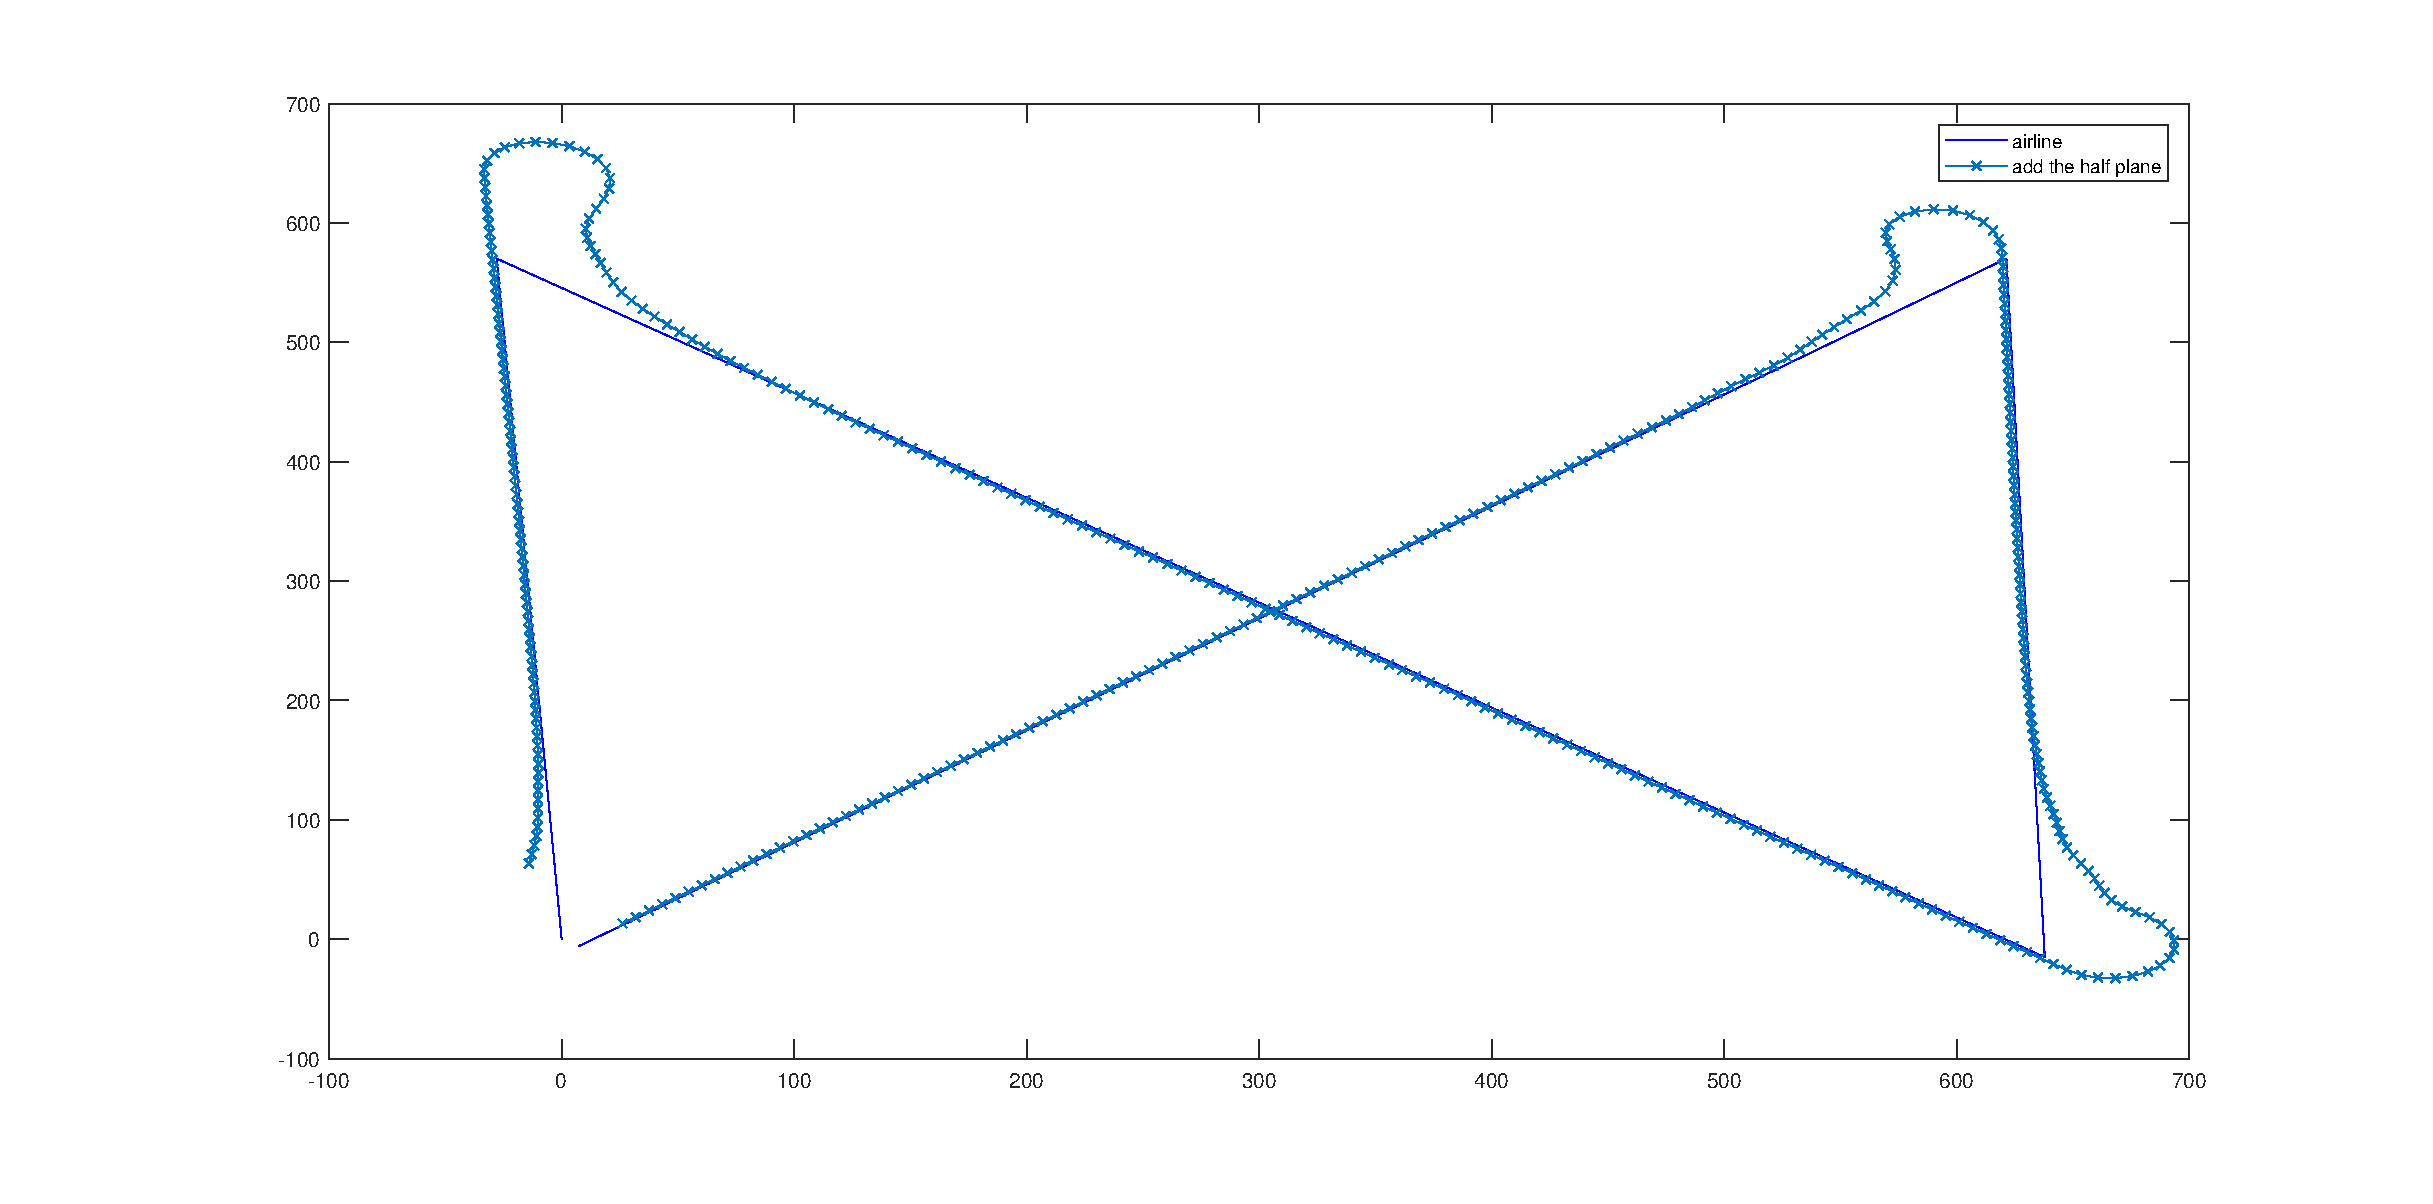
\includegraphics[width=\textwidth]{pictures/eps/algorithm5.eps}
                \label{straight_}
            \end{minipage}
        }
        \caption{straight line}
    \end{figure}
    \begin{figure}[h]
        \centering
        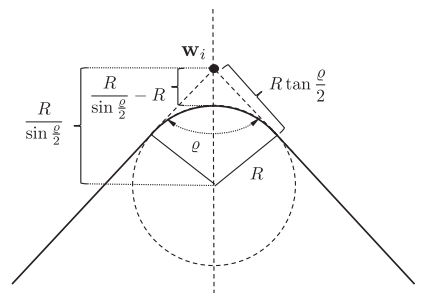
\includegraphics[width=0.5\textwidth]{pictures/algo6_2.png}
        \caption{插入fillet}
        \label{figure:alg6}
    \end{figure}
    \par 无人机从航点$w_{i-1}$到$w_{i}$的飞行过程中,若到达两条航线所生成的半平面,则认为到达了目标航点,
    航线进行切换。飞行控制逻辑包含直线飞行控制和盘旋飞行控制,在直线飞行的过程中,
    航点切换依附着算法\ref{algo5:ref}(航点控制逻辑1)。
    
    第一次执行该算法时候,需要初始化i的值,让其等于2,见\ref{algo5:ref:init};UAV会执行航线$\overline{w_{i-1}w_{i}}$,在算法第4、5行分别定义针对当前执行航点的$r$和$q$,第6行定义了下一条航线的单位方向向量,第7行是航线 $\overline{w_{i-1}w_{i}}$ 和 $\overline{w_{i}w_{i+1}}$ 所生成半平面的法向量,8行到10行进行位置判定,若满足某个关系式,即若无人机穿过半平面,
    那么就要切换航点,执行下一条航线,直到最后一个航点序列号减一。
    \begin{algorithm}[h]
            \caption{Follow Waypoints:(r, q)=followWpp($\textit{W}$, p)}
            \label{algo5:ref}
            \begin{algorithmic}[1]
                \ENSURE Waypoints path $\textit{W}$ = $\left\{ w_{1}, \dots, w_{N} \right\}$, MAV position p=$(p_{n}, p_{e}, p_{d})^{T}$.
                \REQUIRE N $\geq$ 3
                \IF {New waypoints path $\textit{W}$ is received}
                    \STATE Initialize waypoint index: $i$ $\gets$ 2
                    \label{algo5:ref:init}
                \ENDIF
                \STATE $r$ $\gets$ $w_{i-1}$

                \STATE $q_{i-1}$ $\gets$ $\frac{w_{i}-w_{i-1}}{\lVert w_{i}-w_{i-1} \rVert}$
                \STATE $q_{i}$ $\gets$ $\frac{w_{i+1}-w_{i}}{\lVert w_{i+1}-w_{i} \rVert}$
                \STATE $n_{i}$ $\gets$ $\frac{q_{i-1}+q_{i}}{\lVert \| q_{i-1}+q_{i} \rVert}$
                \IF {$p$ $\in$ $\textit{H}(w_{i},n_{i})$}
                    \STATE Increment $i$ $\gets$ $\left(i+1\right)$ until $i$ = $N$ - 1
                \ENDIF
                \RETURN $r$, $q$=$q_{i-1}$ at each time step.  % this command shows "Output"
            \end{algorithmic}
        \end{algorithm}

        \par 算法\ref{algo5:ref}产生的飞行效果如图\ref{straight_}所示,
        很明显,但在直线飞行航点之间切换的时候,因忽略转弯时无人机初始动量的问题,造成了一段很长的转换缓冲距离,致使飞行效果很差,航线不平滑。
    \subsection{航点控制逻辑2}
        \par 对其优化有两种方法, 一是当无人机当前的位置在当前执行的航线上的投影到该航线的起点的\textcolor{blue}{距离占整个比重的90\%}的时候, 进行航点切换;
    
    另外一个较优的改进方法是为其增加一个\textcolor{blue}{圆角(fillet)},如图\ref{fig:algor6}所示,在航点 $w_{i}$ 附近,生成一个盘旋中心,
 让其使得无人机在执行该航点的时候,以圆弧的方式进入到下一条航线,这么航线飞行出来的效果较好。
 定义航线$\overline{w_{i-1}w_{i}}$ 和$\overline{w_{i}w_{i+1}}$的角度为 $\varrho$:
 \begin{figure}[h]
    \centering
    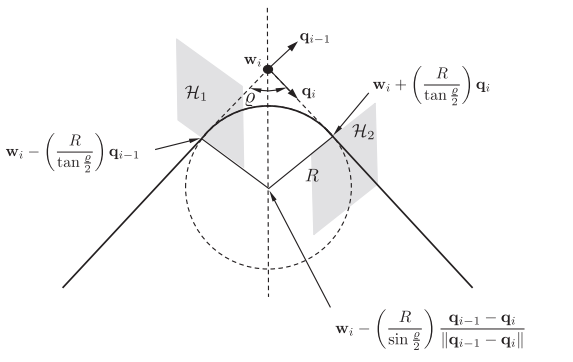
\includegraphics[width=0.6\textwidth]{pictures/algo6_3.png}
    \caption{将半平面和fillet进行结合}
    \label{fig:algor6}
\end{figure}
    \begin{equation}
        \varrho \triangleq cos^{-1}(-q_{i-1}^{T}q_{i})
    \end{equation}
    
    \begin{algorithm}[h]
            \caption{Follow Waypoints with Fillet:(flag, r, q, c, $\rho$, $\lambda$)=followWppFillet($\textit{W}$, p, $R$)}
            \label{algo6:ref}
            \begin{algorithmic}[1]
                \ENSURE Waypoints path $\textit{W}$ = $\left\{ w_{1}, \dots, w_{N} \right\}$, MAV position p=$(p_{n}, p_{e}, p_{d})^{T}$, fillet radius $R$
                \REQUIRE N $\geq$ 3
                \IF {New waypoints path $\textit{W}$ is received}
                    \STATE Initialize waypoint index: $i$ $\gets$ 2, and state machine: state $\gets$ 1
                \ENDIF
                \STATE $q_{i-1}$ $\gets$ $\frac{w_{i}-w_{i-1}}{\lVert w_{i}-w_{i-1} \rVert}$
                \STATE $q_{i}$ $\gets$ $\frac{w_{i+1}-w_{i}}{\lVert w_{i+1}-w_{i} \rVert}$
                \STATE $\varrho$ $\gets$ $cos^{-1}(-q_{i-1}^{T}q_{i})$
                \IF {state = 1}
                    \STATE flag $\gets$ 1
                    \STATE $r$ $\gets$ $w_{i-1}$
                    \STATE $q$ $\gets$ $q_{i-1}$
                    \STATE $z$ $\gets$ $w_{i} - \frac{R}{tan(\frac{\varrho}{2})}q_{i-1}$

                    \IF {$p$ $\in$ $\textit{H}(z,q_{i-1})$}
                        \STATE state $\gets$ 2
                    \ENDIF
                \ELSIF{state = 2}
                    \STATE flag $\gets$ 2
                    \STATE $c$ $\gets$ $w_{i} - \frac{R}{sin(\frac{\varrho}{2})}\frac{q_{i-1}-q_{i}}{\lVert q_{i-1}-q_{i} \rVert}$
                    \STATE $\rho$ $\gets$ $R$
                    \STATE $\lambda$ $\gets$ $sign(q_{i-1,n}q_{i,e}-q_{i-1,e}q_{i,n})$
                    \STATE $z$ $\gets$ $w_{i} + \frac{R}{tan(\frac{\varrho}{2})}q_{i}$
                    \IF {$p$ $\in$ $\textit{H}(z,q_{i})$}
                        \STATE $i$ $\gets$ $\left(i+1\right)$ until $i$ = $N$ - 1
                        \STATE state $\gets$ 1
                    \ENDIF
                \ENDIF
                \RETURN flag, $r$, $q$, $c$, $\rho$,$\lambda$.  % this command shows "Output"
            \end{algorithmic}
        \end{algorithm}
在图\ref{figure:alg6}中,假定fillet的半径为R,那么圆弧和两条航线的切点距航点$w_{i}$的距离为$\frac{R}{tan(\frac{\varrho}{2})}$
    且航点$w_{i}$和fillet的中心的距离是$\frac{R}{sin(\frac{\varrho}{2})}$,所以航点$w_{i}$距圆角fillet的最短距离为$\frac{R}{sin(\frac{\varrho}{2})}$ - $R$.
    为了让其直线控制逻辑和圆弧控制逻辑\upcite{8}更好的结合,对此也引进来了"半平面"。
    在图\ref{fig:algor6}中,
    定义了两个半平面 \textit{$H_{1}$} 和 \textit{$H_{2}$}。飞机在未进入半平面 \textit{$H_{1}$}
    的时候,执行直线控制逻辑;当进入到 \textit{$H_{1}$} 的时候,执行圆弧控制逻辑,此时,圆弧的中心是 $c$,半径是 $\rho$;直到无人机进入 \textit{$H_{2}$} ,切换到直线控制逻辑。
    在算法\ref{algo6:ref}(航点控制逻辑2)中,给出了详细的逻辑梳理。
    圆角的中心 $c$, 第一个半平面、第二半平面与圆角相交的点 $r_{1}$ 和 $r_{2}$ 定义如下:
        \begin{align}
            &c = w_{i} - \frac{R}{sin(\frac{\varrho}{2})} \frac{q_{i-1}-q_{i}}{\lVert q_{i-1}-q_{i} \rVert} \\
            &r_{1} = w_{i} - \left( \frac{R}{tan(\frac{\varrho}{2})} \right)q_{i-1} \\
            &r_{2} = w_{i} + \left( \frac{R}{tan(\frac{\varrho}{2})} \right)q_{i}
        \end{align}
    \par其中的向量 $q_{i-1}$ 和 $q_{i}$ 分别为两条航线的单位方向向量。算法\ref{algo6:ref}中,若一条新的航线被接收,那么航点序列号和state的值也会在第2行进行更新,向量$q_{i-1}$ 和 $q_{i}$,以及$\varrho$在4到6行计算;
    当state = 1的时候,调用直线控制逻辑,执行航线 $\overline{w_{i-1}w_{i}}$,同时计算相对应的 $r$ 和 $q$,在第11到14行判断是否到达第一个半平面;若无人机穿过第一个半平面,朝着第二个半平面飞去的时候,state = 2,执行曲线控制逻辑,对应的圆心为$c$,半径为$\rho$,飞行的方向(逆时针,或顺时针)为$\lambda$;若无人机穿过第二个半平面,则state赋值为1,执行直线控制逻辑。

    
    \subsection{算法优化} 
    算法\ref{algo5:ref}和算法\ref{algo6:ref}执行效果对比如图\ref{algo5_com_6}所示, 图\ref{5_6_bigger}是将右下角转弯轨迹放大之后得到的. 很显然, 从总体路径长度最优的角度来看, 后者的总体路径长度要明显比前者总体路径长度短很多, 执行效率也会优于前者.
    \begin{figure}[h]
        \centering
        \subfigure[]{
            \begin{minipage}[t]{0.48\linewidth}
                \centering
                    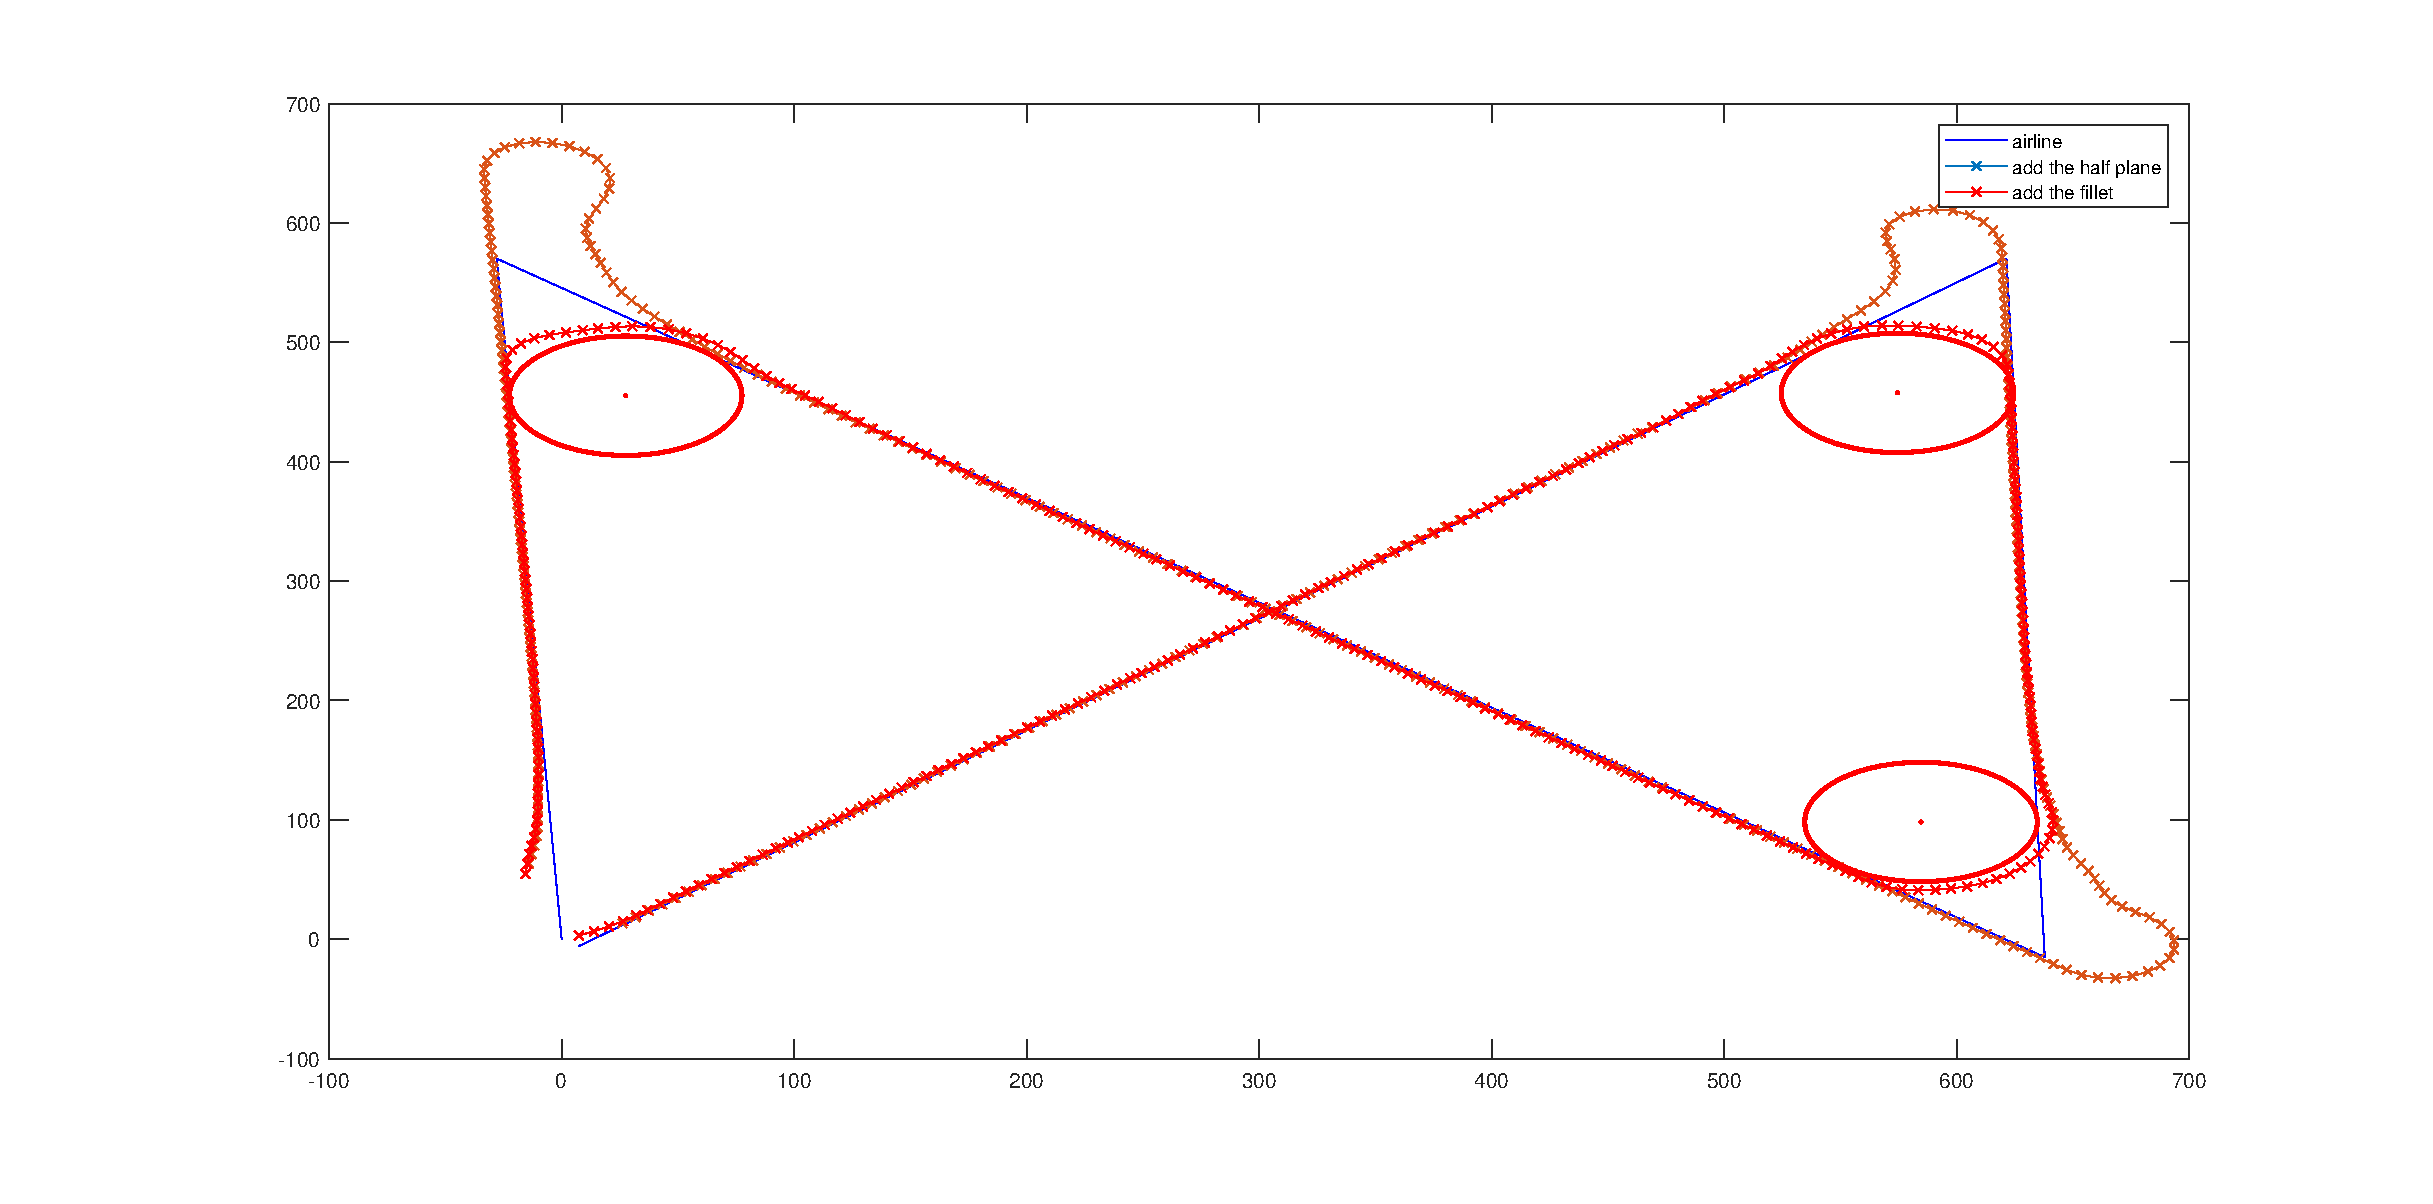
\includegraphics[width=\textwidth]{pictures/eps/algorithm5_6.eps}
                \label{algo5_com_6}
            \end{minipage}
        }
        \subfigure[]{
            \begin{minipage}[t]{0.48\linewidth}
                \centering
                    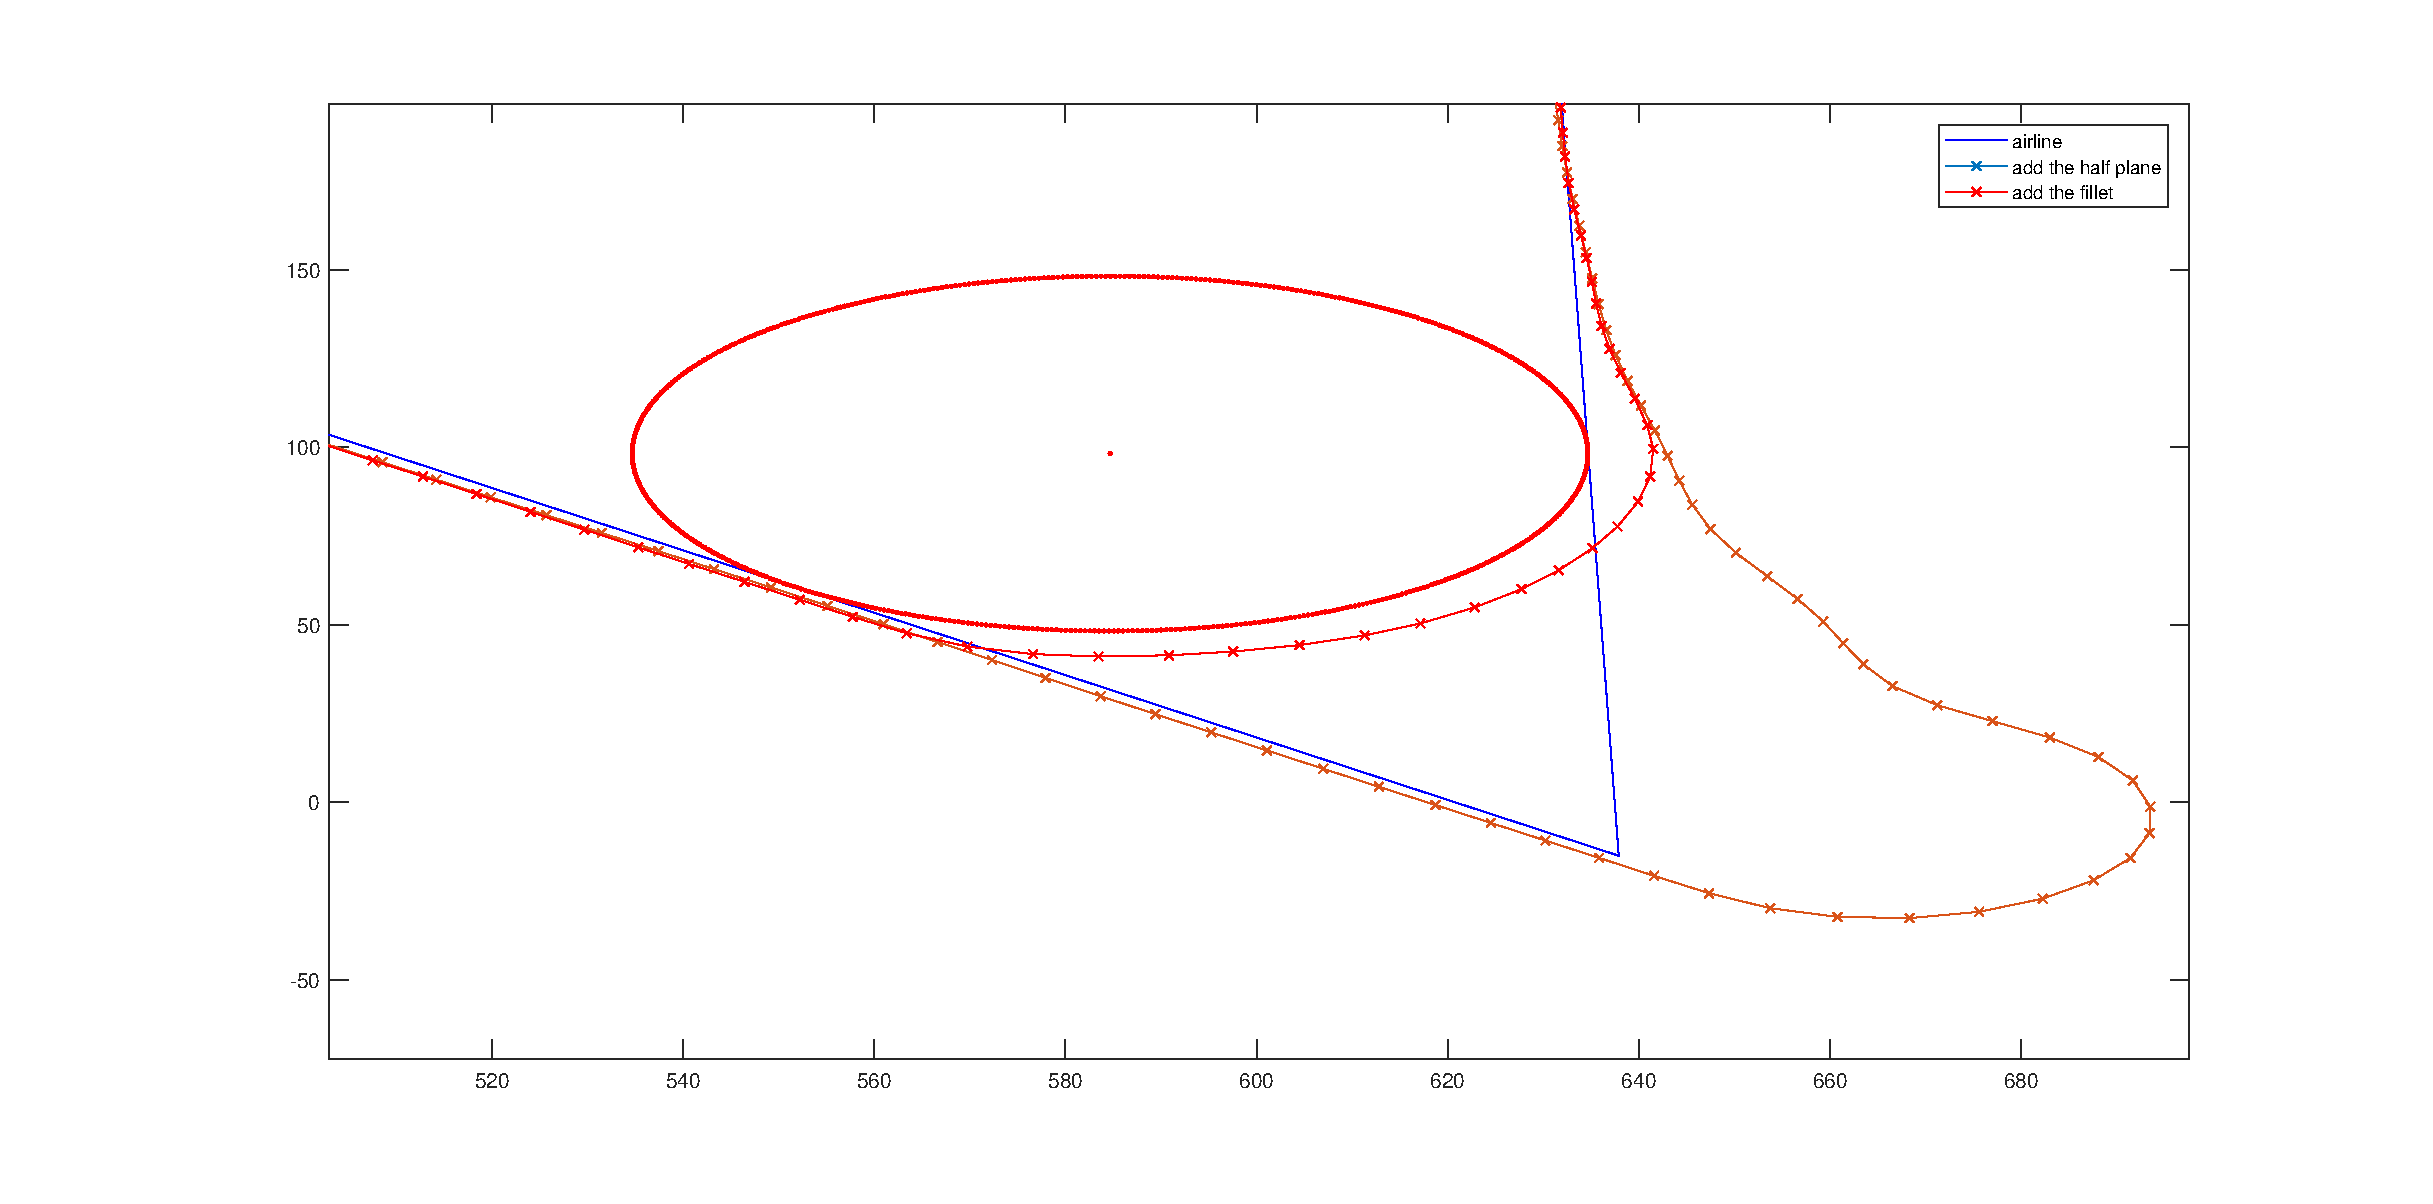
\includegraphics[width=\textwidth]{pictures/eps/algorithm5_6_1.eps}
                \label{5_6_bigger}
            \end{minipage}
        }
        \caption{comparing}
    \end{figure}
    尽管如此, 算法\ref{algo6:ref}在转弯的时候, 对初试惯性动量考虑的不太周到, 存在一些瑕疵, 如图\ref{fig:algo6}所示.
    虽然在算法\ref{algo6:ref}中, 模型建立是以fillet和航线相切的情况来考虑的, 但在仿真平台中, 无人机的并不是以期望空速来飞行, 而是以期望空速(airspeed)和风速(wind speed)叠加之后形成的地速(ground speed)来飞行. 由于风速大小的不确定性, 造成了飞行效果差强人意.
    \begin{figure}[htbp]
        \centering
        \subfigure[]{
            \begin{minipage}[t]{0.48\linewidth}
                \centering
                    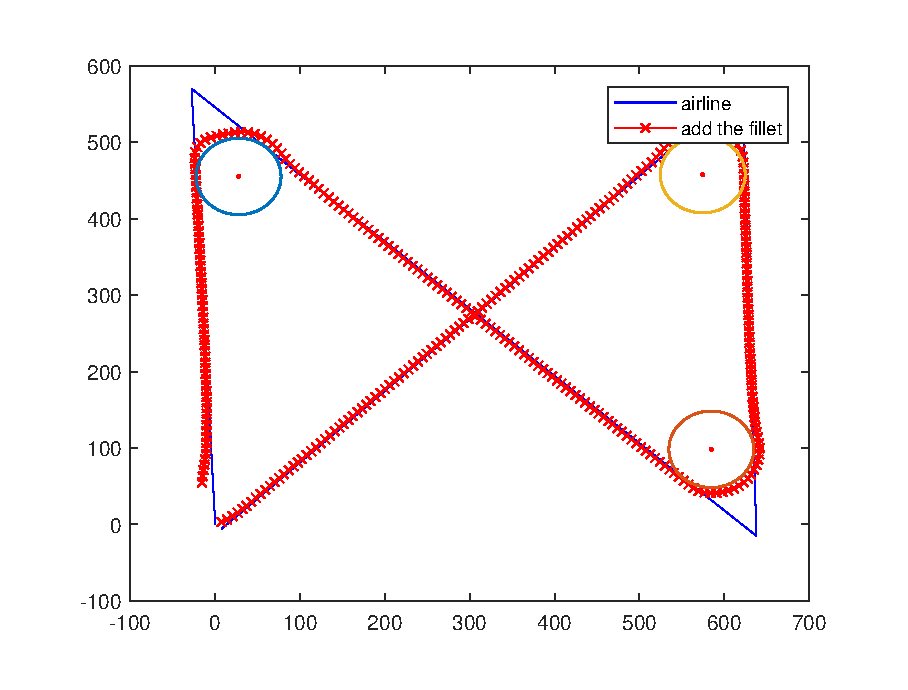
\includegraphics[width=0.8\textwidth]{pictures/eps/algorithm6.eps}
                \label{fig:algo6}
            \end{minipage}
        }
        \subfigure[]{
            \begin{minipage}[t]{0.48\linewidth}
                \centering
                    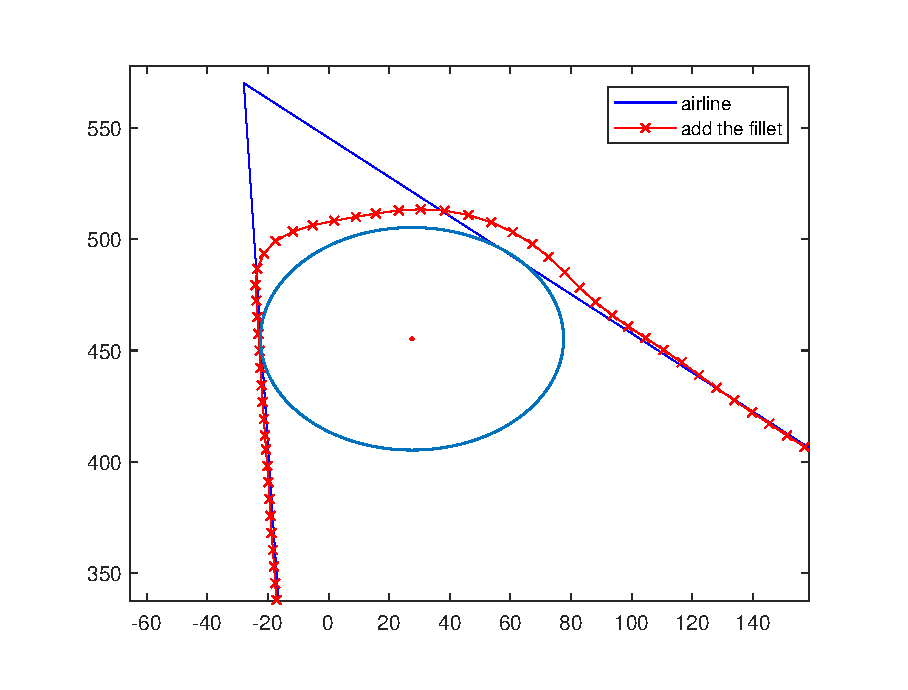
\includegraphics[width=0.8\textwidth]{pictures/eps/algorithm6_1.eps}
                \label{fig:algo6_1}
            \end{minipage}
        }
        \\
        \subfigure[]{
            \begin{minipage}[t]{0.48\linewidth}
                \centering
                    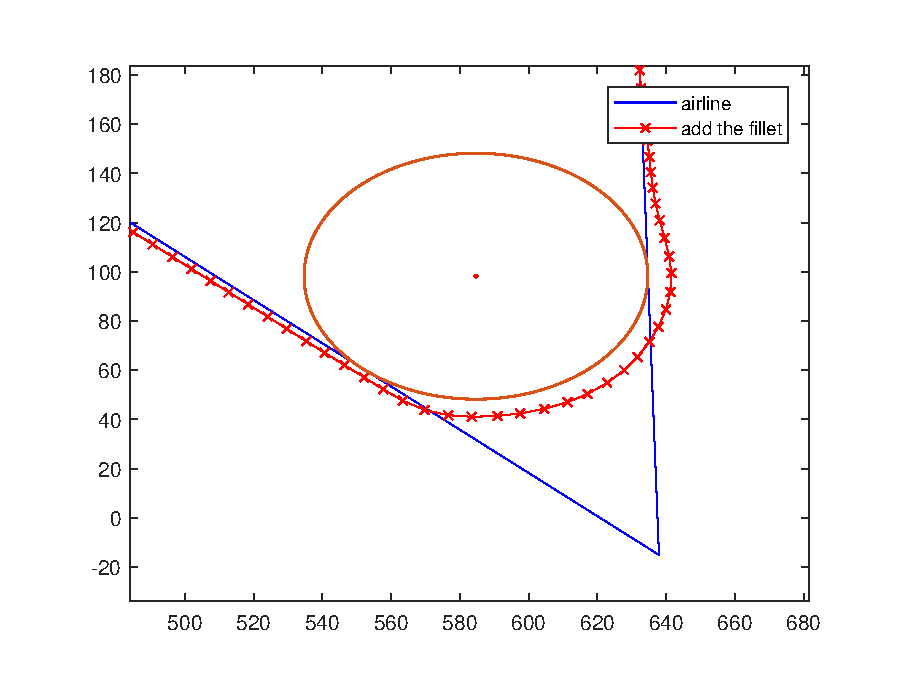
\includegraphics[width=0.8\textwidth]{pictures/eps/algorithm6_2.eps}
                \label{fig:algo6_2}
            \end{minipage}
        }
        \subfigure[]{
            \begin{minipage}[t]{0.48\linewidth}
                \centering
                    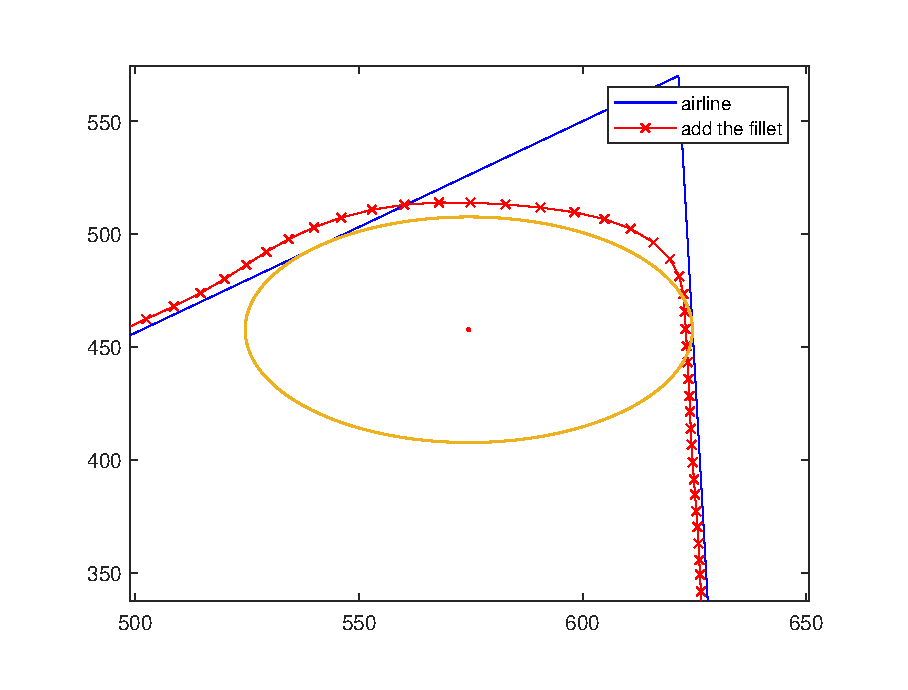
\includegraphics[width=0.8\textwidth]{pictures/eps/algorithm6_3.eps}
                \label{fig:algo6_3}
            \end{minipage}
        }
        \caption{algorithm6}
    \end{figure}
 
    对此提出了一个算法的改进. 根据图\ref{fig:algo6_1}, \ref{fig:algo6_2}, \ref{fig:algo6_3}显示, 超出航线的那一小部分还是由于惯性动量导致的, 所以在这里我们需要提前来进行航先切换, 从而留出一部分来减弱惯性动量, 让转弯轨迹更加的圆滑, 航线执行总的距离更小. 故对算法\ref{algo6:ref}进行了改进, 从而得到了算法\ref{algo6_opti:ref}.   
    \begin{figure}[htbp]
        \centering
        \subfigure[]{
            \begin{minipage}[t]{0.48\linewidth}
                \centering
                    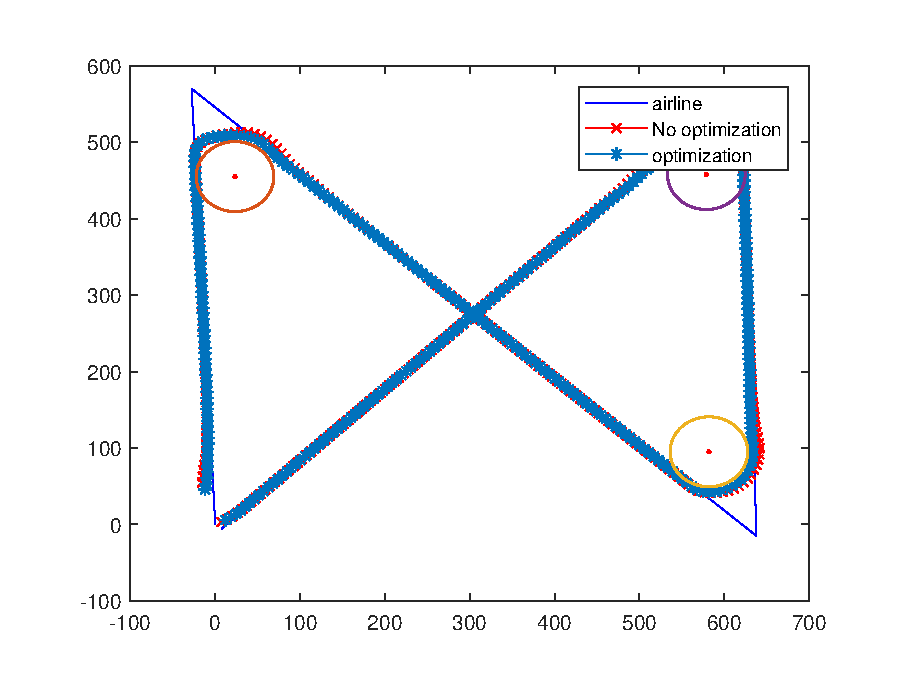
\includegraphics[width=0.7\textwidth]{pictures/eps/algorithm7.eps}
                \label{fig:algo7}
            \end{minipage}
        }
        \subfigure[]{
            \begin{minipage}[t]{0.48\linewidth}
                \centering
                    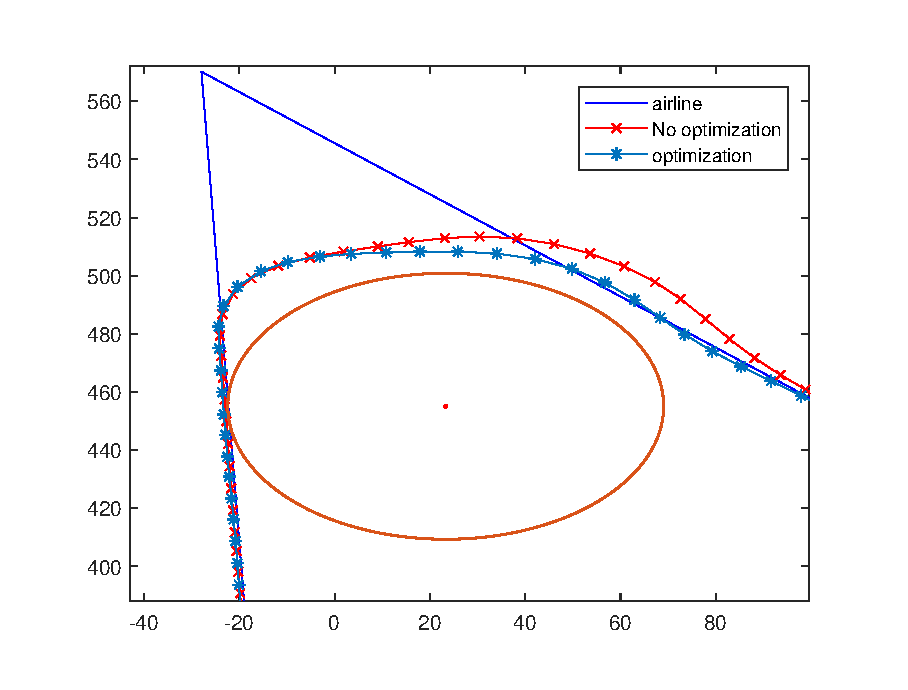
\includegraphics[width=0.7\textwidth]{pictures/eps/algorithm7_1.eps}
                \label{fig:algo7_1}
            \end{minipage}
        }
        \\
        \subfigure[]{
            \begin{minipage}[t]{0.48\linewidth}
                \centering
                    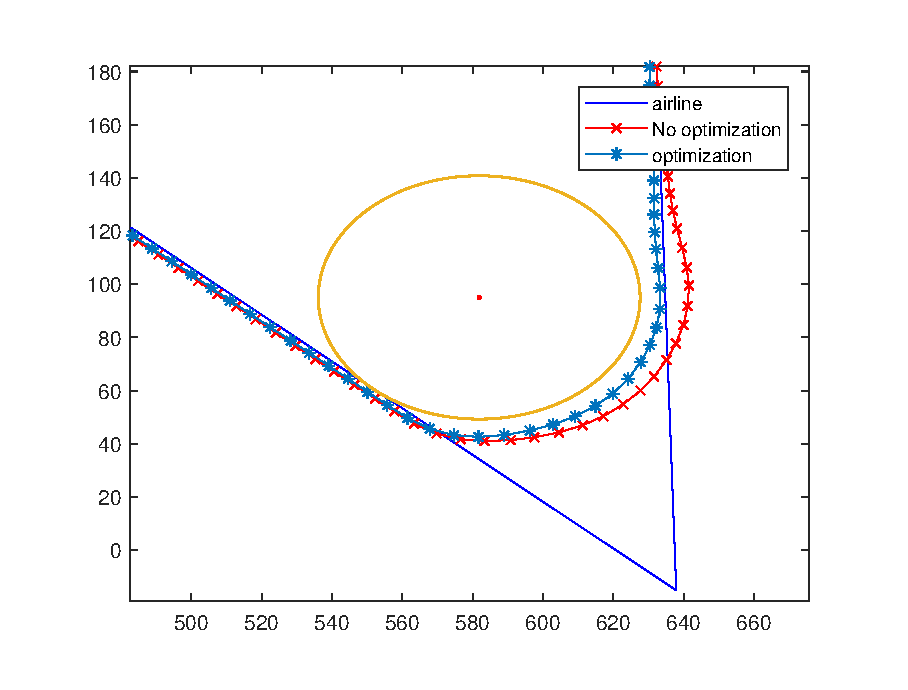
\includegraphics[width=0.7\textwidth]{pictures/eps/algorithm7_2.eps}
                \label{fig:algo7_2}
            \end{minipage}
        }
        \subfigure[]{
            \begin{minipage}[t]{0.48\linewidth}
                \centering
                    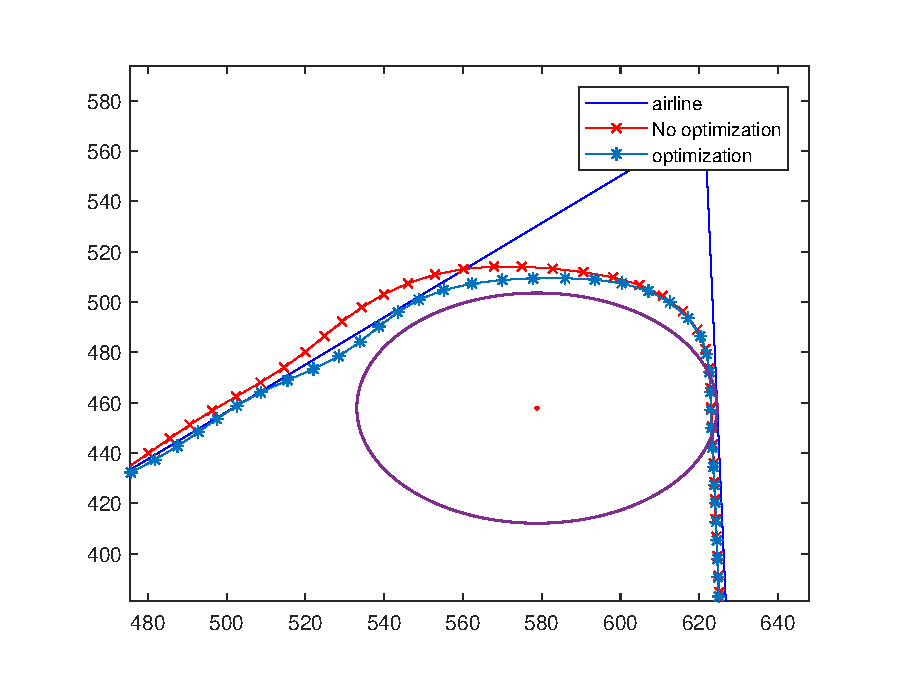
\includegraphics[width=0.7\textwidth]{pictures/eps/algorithm7_3.eps}
                \label{fig:algo7_3}
            \end{minipage}
        }
        \caption{algorithm6 comparing 1}
    \end{figure}
    
    \par 算法中, 在\ref{algo7_z1}行, 保存第一个半平面与航线$\overline{w_{i-1}w_{i}}$的交点$z$为$z_{1}$, 
    当进入第一个半平面的时候,state = 2,执行曲线控制逻辑,对应的圆心为第\ref{new_center}行所示的$c$, 其中半径进行了一定比例的缩放,已到达保留一定的距离来消耗无人机初始惯性动量的目的。第20行和22行,对应的R都进行了比例缩放,其中第20行是为fillet center设置半径,第22行是计算新的第二个半平面和下一条航线的新交点;第23行判断是否到达第二个半平面,若到达则切换航线,state重新设置为1,执行直线控制逻辑;反之继续执行当前航线。
    前后算法比对的效果图如图\ref{fig:algo7}所示。
    \begin{algorithm}[t] % 算法6 的优化
        \caption{Follow Waypoints with Fillet:(flag, r, q, c, $\rho$, $\lambda$)=followWppFillet($\textit{W}$, p, $R$)}
        \label{algo6_opti:ref}
        \begin{algorithmic}[1]
            \ENSURE Waypoints path $\textit{W}$ = $\left\{ w_{1}, \dots, w_{N} \right\}$, MAV position p=$(p_{n}, p_{e}, p_{d})^{T}$, fillet radius $R$
            \REQUIRE N $\geq$ 3
            \IF {New waypoints path $\textit{W}$ is received}
                \STATE Initialize waypoint index: $i$ $\gets$ 2, and state machine: state $\gets$ 1
            \ENDIF
            \STATE $q_{i-1}$ $\gets$ $\frac{w_{i}-w_{i-1}}{\lVert w_{i}-w_{i-1} \rVert}$
            \STATE $q_{i}$ $\gets$ $\frac{w_{i+1}-w_{i}}{\lVert w_{i+1}-w_{i} \rVert}$
            \STATE $\varrho$ $\gets$ $cos^{-1}(-q_{i-1}^{T}q_{i})$
            \IF {state = 1}
                \STATE flag $\gets$ 1
                \STATE $r$ $\gets$ $w_{i-1}$
                \STATE $q$ $\gets$ $q_{i-1}$
                \STATE $z$ $\gets$ $w_{i} - \frac{R}{tan(\frac{\varrho}{2})}q_{i-1}$
                \STATE $z_{1}$ $\gets$ $z$     \label{algo7_z1}   
                \IF {$p$ $\in$ $\textit{H}(z,q_{i-1})$}
                    \STATE state $\gets$ 2
                \ENDIF
            \ELSIF{state = 2}
                \STATE flag $\gets$ 2
                
                % 计算新的 center >>>>>>>>>>>>>>>>> 
                \STATE $c$ $\gets$ $w_{i} - \frac{R}{sin(\frac{\varrho}{2})}\frac{q_{i-1}-q_{i}}{\lVert q_{i-1}-q_{i} \rVert}$
                \STATE $c$ $\gets$ $z_{1} + \frac{c-z_{1}}{\lVert c-z_{1}\rVert}*0.915R$ %  \frac{R}{sin(\frac{\varrho}{2})}\frac{q_{i-1}-q_{i}}{\lVert \| q_{i-1}-q_{i} \rVert}$
                \label{new_center}
                \STATE $\rho$ $\gets$ $0.915R$
                % <<<<<<<<<<<<<<<<< 计算新的 center

                \STATE $\lambda$ $\gets$ $sign(q_{i-1,n}q_{i,e}-q_{i-1,e}q_{i,n})$
                \STATE $z_{2}$ $\gets$ $w_{i} + \frac{1}{tan(\frac{\varrho}{2})}*0.915R*q_{i}$
                \IF {$p$ $\in$ $\textit{H}(z,q_{i})$}
                    \STATE $i$ $\gets$ $\left(i+1\right)$ until $i$ = $N$ - 1
                    \STATE state $\gets$ 1
                \ENDIF
            \ENDIF
            \RETURN flag, $r$, $q$, $c$, $\rho$,$\lambda$.  % this command shows "Output"
        \end{algorithmic}
    \end{algorithm}
    \subsubsection{误差分析}
    \begin{center} 
        \begin{table}[H]
            \caption{误差分析表}
            \label{tab1}
            \begin{tabular}{c|c|c|c|c}
                \hline
                & 第一段(*150)& 第二段((*130))& 第三段(*120) &总和 \\
                \hline
                优化之前 &9.506485437269829& 13.459338133308067& 12.517388189403794 & 11.694433389122446 \\
                \hline
                优化之后 &9.307437579575690& 2.896129449605189& 7.097844734906930 & 6.560884583934650 \\
                \hline
                % \caption{误差分析表}
            \end{tabular} 
        \end{table}   
    \end{center}
    
    通过计算超出航线部分的点到航线的垂直距离,即偏离航线的误差,来判定算法是否优化。算法优化之前和优化之后误差分析如\ref{tab1}所示。
    最终计算得到的总的偏差由11.7减少到6.6,效果优化了78\%,足以可见算法\ref{algo6_opti:ref}较之前算法具有很好的效用性。

    \section{制导控制} 
        \subsection{集群(主机)控制逻辑}
            \subsubsection{OFFBOARD}
            OFFBOARD模式控制下主要存在两种控制算法: TECS 和 L1控制律, 其中TECS就是利用势能和动能总和不变来根据期望高度和空速计算出期望pitch值以及期望throttle值;
            L1制导算法,就是在航线上选择与无人机距离为L1的参考点,然后根据速度方向与到参考点连线方向之间的夹角计算横向加速度, 进而求得滚转roll, 实现航线跟踪。\par
            这两者的算法都是从PX4内部剥离出来, 在OFFBOARD模式下进行的逻辑控制. 
            \clearpage
            \subsubsection{RC}
            \textcolor{red}{直线控制逻辑\ref{alg:strai}}
            \begin{figure}[htpb]
                \centering
                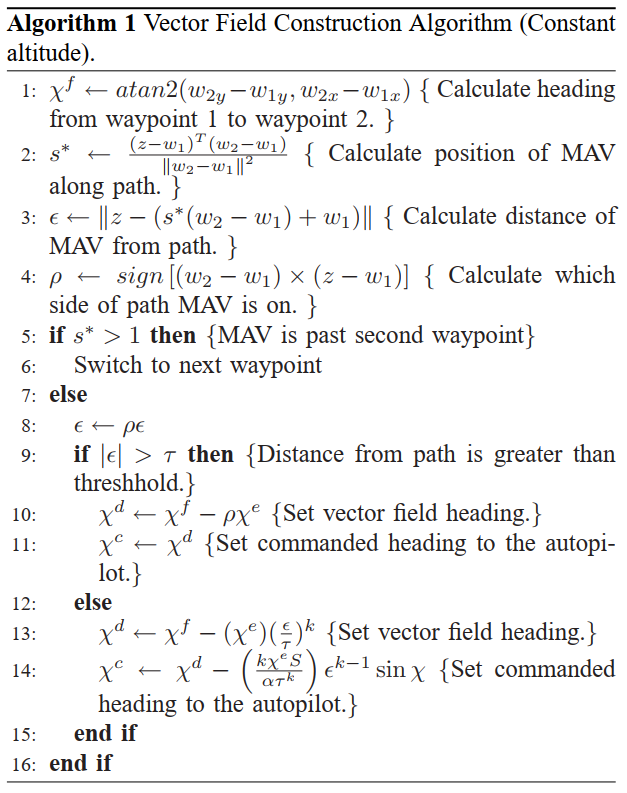
\includegraphics[width=0.5\textwidth]{pictures/algorithm/straight.png}
                \caption{直线控制逻辑}
                \label{alg:strai}
            \end{figure}
            
            \textcolor{red}{盘旋控制逻辑\ref{alg:loiter}}
            \begin{figure}[htpb]
                \centering
                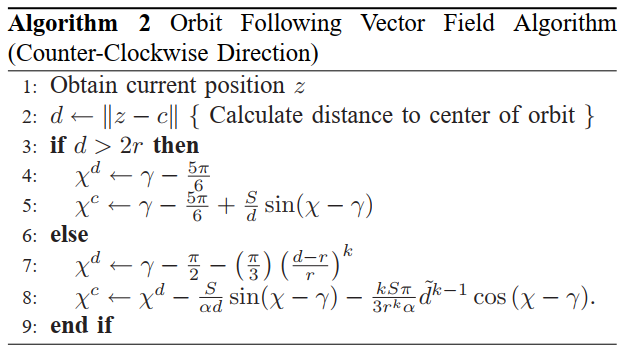
\includegraphics[width=0.5\textwidth]{pictures/algorithm/loiter.png}
                \caption{盘旋控制逻辑}
                \label{alg:loiter}
            \end{figure}
            \clearpage
        \subsection{编队控制逻辑}
        从机的导航子系统中, 会根据当前飞机的位置, 以及主机的当前位置以及编队的gap值, 计算出从机期望位置点. 下发给从机的制导控制器, 进行编队, 其中的算法逻辑如下: 
        \begin{algorithm}[htpb]
            \caption{Formation control:($\psi$, throttle)}
            \begin{algorithmic}[1]
                \ENSURE (followerFinalPoint, followerPosition, followerHeading), (leaderHeading, leaderHeadingCommanded, groundSpeedLeader)
                
                \STATE $followerFinalPoint_{Proj}.x$ $\gets$ $followerFinalPoint.x + cos(leaderHeadingCommanded)$
                \STATE $followerFinalPoint_{Proj}.y$ $\gets$ $followerFinalPoint.y + sin(leaderHeadingCommanded)$
                \STATE $A$ $\gets$ $(followerFinalPoint.x - followerPosition.x) * cos(followerHeading)$
                \STATE $B$ $\gets$ $(followerFinalPoint.y - followerPosition.y) * sin(followerHeading)$
                \STATE $x_{e}$ $\gets$ $A + B$
                \STATE $\chi_e$ $\gets$ $leaderHeading - followerHeading$
                \STATE $followerDistance$ $\gets$ $followerFinalPoint - followerPosition$
                \IF {$followerDistance$ $\textgreater$ $threshold$}
                    \STATE $headingSetpoint$ $\gets$ $atan2(\frac{followerFinalPoint.y - followerPosition.y}{ followerFinalPoint.x - followerPosition.x})$
                    \STATE $groundSpeedSetpoint$ $\gets$ $2*groundSpeedLeader$
                \ELSIF{$followerDistance$ $\leq$ $threshold$}
                    \STATE $groundSpeedSetpoint$ $\gets$ $c1 * x_e + groundSpeedLeader * cos(chi_e)$
                    \STATE $headingSetpoint$ $\gets$ $leaderHeadingCommanded$ + $side*\chi_{\inf}*(\frac{followerDistance}{threshold}^{k})$; 
                \ENDIF
                \STATE $throttle$ $\gets$ $groundSpeedSetpoint$
                \STATE $\psi$ $\gets$ $headingSetpoint$
                \RETURN ($\psi$, $throttle$).  % this command shows "Output"
            \end{algorithmic}
        \end{algorithm}

        % Point followerFinalPoint_Proj(
        %     followerFinalPoint.x + cos(leaderHeadingCommanded),
        %     followerFinalPoint.y + sin(leaderHeadingCommanded)
        % ); 
    
        % double x_e = ((followerFinalPoint.x - followerPosition.x) * cos(followerHeading))+
        %         ((followerFinalPoint.y -followerPosition.y)*sin(followerHeading));
                
        % double chi_e = leaderHeading - followerHeading;
    
        % int side = (Point::det(
        %             followerFinalPoint-followerFinalPoint_Proj, 
        %             followerPosition-followerFinalPoint_Proj)
        %         ) >= 0 ? 1 : -1;
           
        % /*  >>>>>>>>>>>>>>>>>>>>>>>>>>>>>>>>>>>>>>>>>  */
        % Point position_error = (followerPosition - followerFinalPoint) * 0.5;
        % double distance_error = Point::norm(position_error);
        % int isAdd = side >= 0 ? -1 : 1;
        % isAdd = 0;
        % groundSpeedSetpoint = c1 * x_e + groundSpeedLeader * cos(chi_e) + isAdd * distance_error;
        % /*  <<<<<<<<<<<<<<<<<<<<<<<<<<<<<<<<<<<<<<<<<  */
    
    
        % double followerDistance = Point::norm(followerFinalPoint - followerPosition);
    
        % if(followerDistance > threshold){
        %     headingSetpoint = atan2(followerFinalPoint.y - followerPosition.y, followerFinalPoint.x - followerPosition.x);
        %     groundSpeedSetpoint = 2*groundSpeedLeader;
    
        % }else
        % {
        %     followerDistance = abs(Point::det(followerFinalPoint_Proj -  followerFinalPoint,followerFinalPoint-followerPosition))/Point::norm(followerFinalPoint_Proj-followerFinalPoint);
        %     int side = (Point::det(followerFinalPoint-followerFinalPoint_Proj, followerPosition-followerFinalPoint_Proj)) >= 0 ? 1 : -1;
        %     headingSetpoint = leaderHeadingCommanded + side*chi_infinite*(pow(followerDistance/threshold,k));    
                  
        % }
        \clearpage
    \section{自组织算法}


  \clearpage
  % 硬件开发 
  %   (硬件的使用标准 + 硬件仿真)
  \chapter{仿真}
    \section{软件仿真}
        \subsection{软件准备}
        \subsection{组成部分}
        \subsection{数据流走向}
        \subsection{效果展示}
    \section{硬件仿真}
        \subsection{硬件准备}
        \subsection{组成部分}
        \subsection{数据流走向}
        \subsection{效果展示}
  \clearpage
\end{document}